\appendix
% % Uncomment for sorted glossary definitions
% \printglossaries

\chapter{Additional Experimental Results}
\begin{figure}[p]
    \centering
    
    \makebox[\linewidth][c]{
        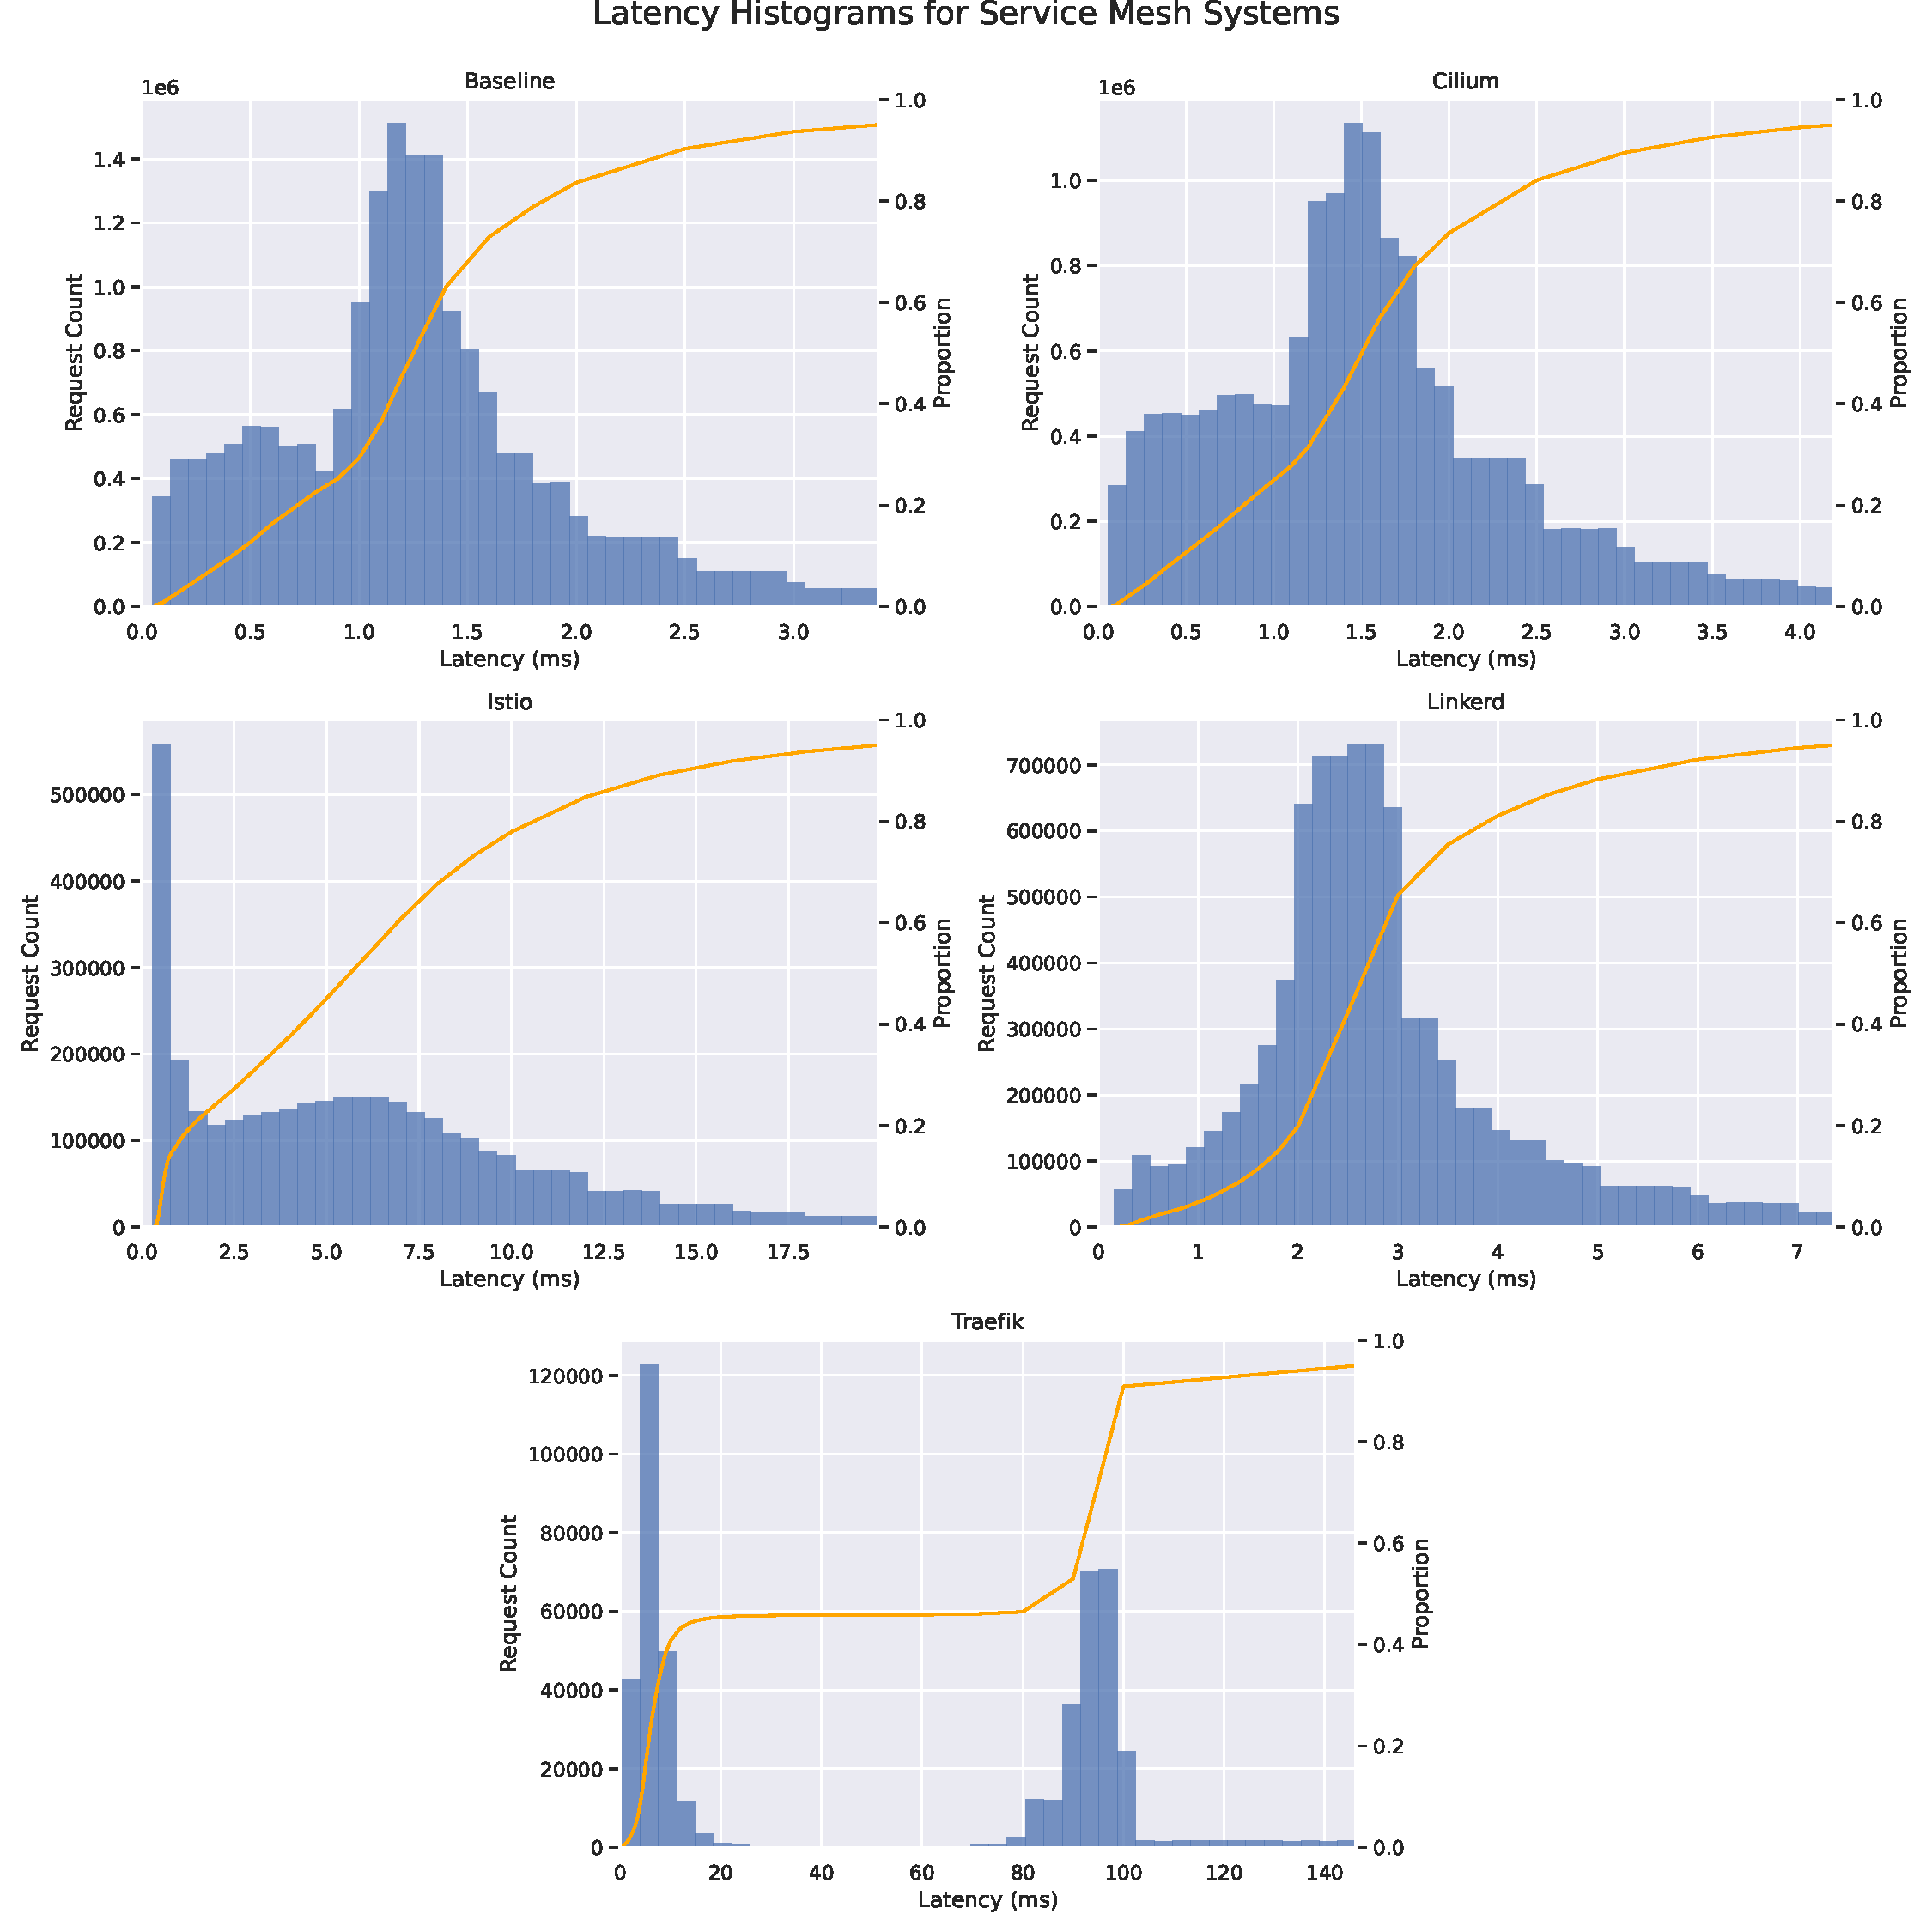
\includegraphics[width=1.2\linewidth]{5_experimental_evaluation/figures/exp-01-distributions-all.pdf}
    }

    \caption[Experiment 1 - Histogram of latencies under maximum load.]{Histogram of latencies under maximum load}
    \label{fig:exp:01:hist-latency-traefik}
\end{figure}


\begin{figure}[p]
    \centering
    
    \makebox[\linewidth][c]{
        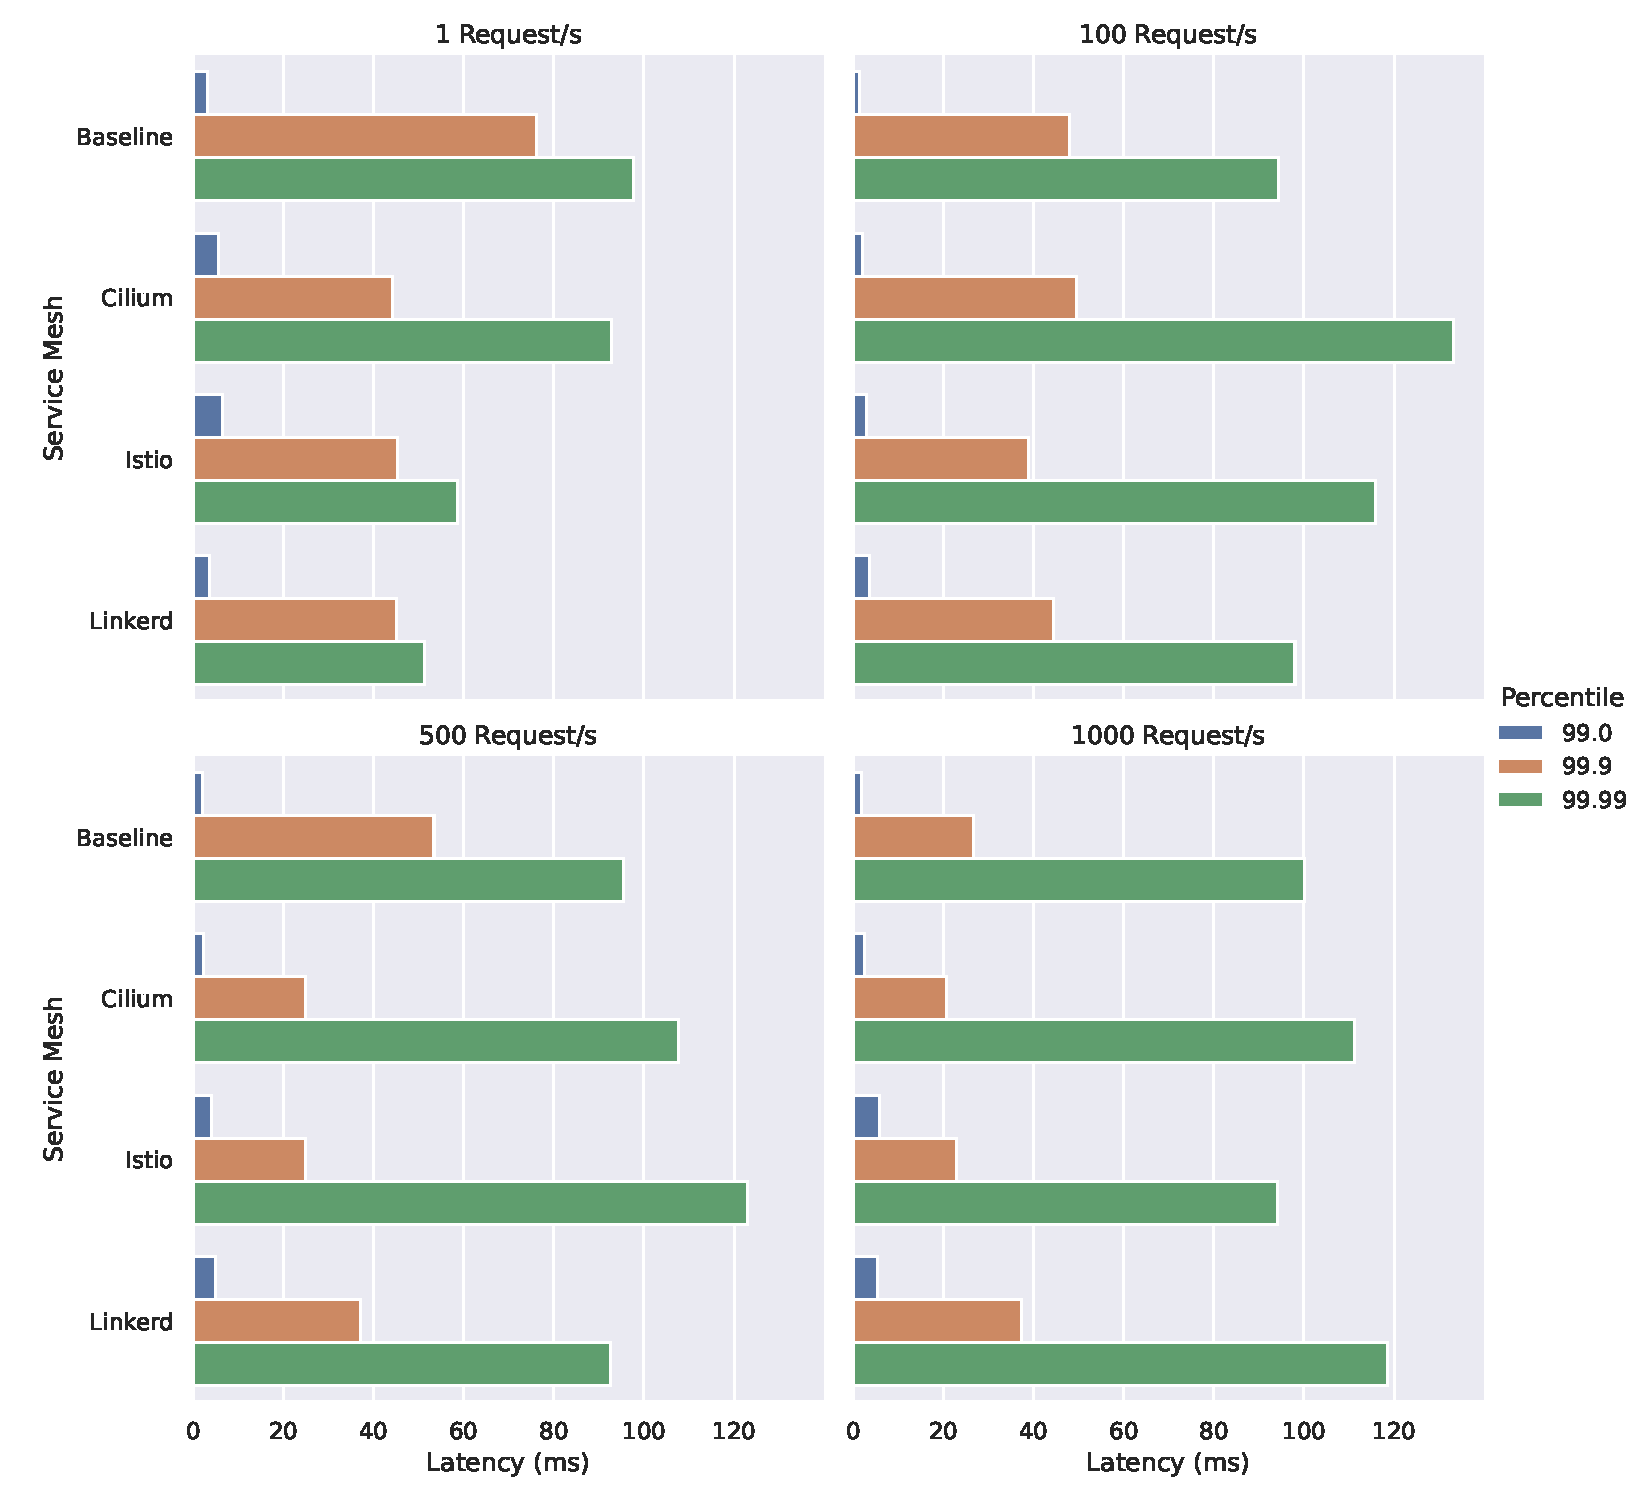
\includegraphics[width=1.3\linewidth]{5_experimental_evaluation/figures/exp-02-tail-latencies-all.pdf}
    }

    \caption[Experiment 2 - Tail end latencies of \gls{sm} systems under varying levels of constant throughput.]{Tail end latencies of \gls{sm} systems under varying levels of constant throughput.}
    
    \label{fig:exp:02:tail-latencies}
\end{figure}



\begin{figure}[p]
    \centering
    
    \makebox[\linewidth][c]{
        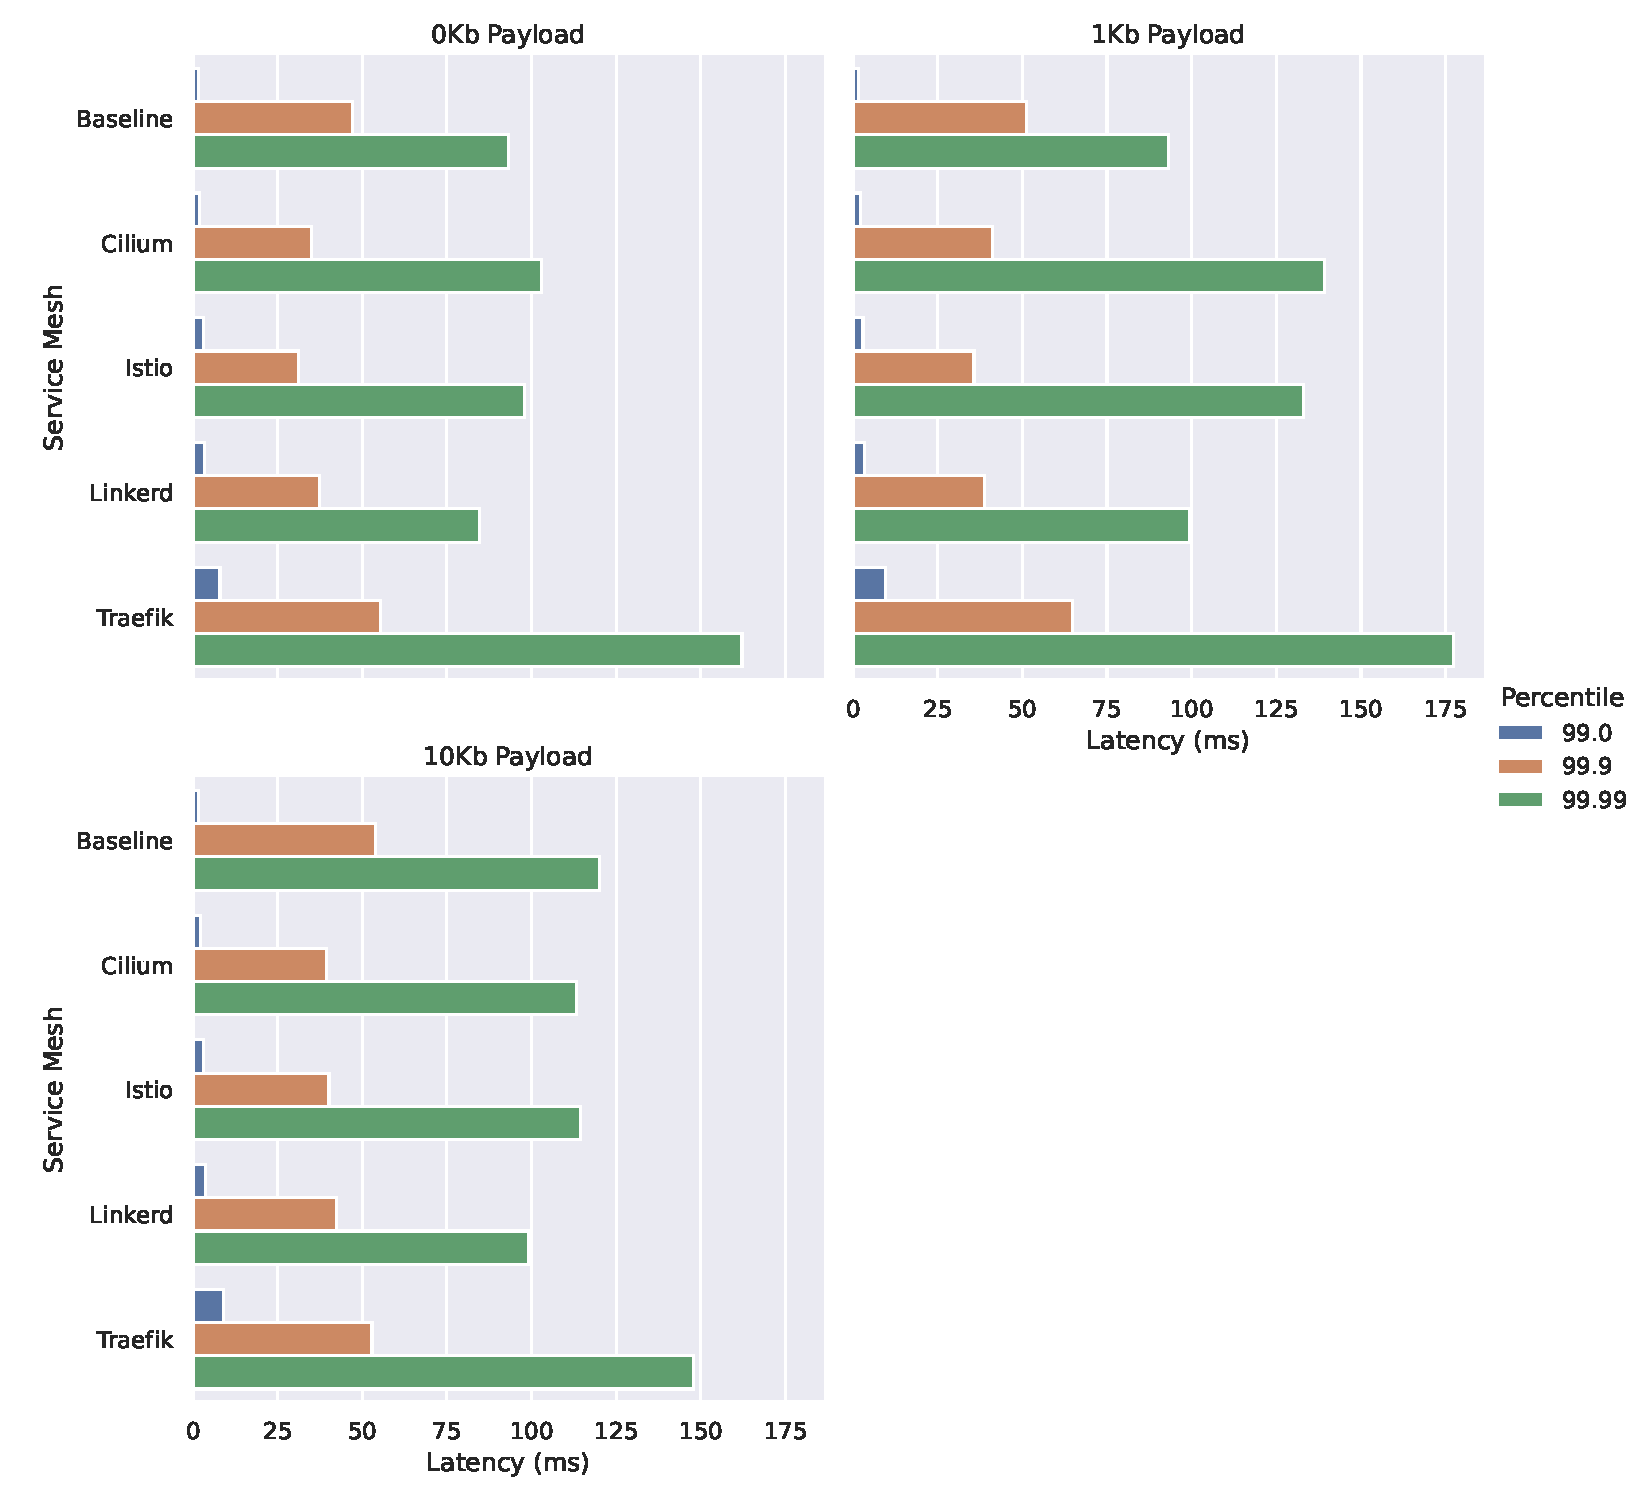
\includegraphics[width=1.3\linewidth]{5_experimental_evaluation/figures/exp-03-tail-latencies-all.pdf}
    }

    \caption[Experiment 3 - Tail end latencies of \gls{sm} systems when experiencing varying application payload sizes.]{Tail end latencies of \gls{sm} systems when experiencing varying application payload sizes.}
    
    \label{fig:exp:03:tail-latencies}
\end{figure}

